\documentclass[10pt,twocolumn]{article}

\usepackage[small,compact]{titlesec} %http://gurmeet.net/computer-science/latex-tips-n-tricks-for-conference-papers/
\usepackage{microtype}
\usepackage{graphicx}

%%%%%%%%%%%%%%%%%%%%%%%%%%%%%% Margins
\setlength{\columnsep}{0.25in}
\usepackage[top=0.8in,bottom=0.8in,left=0.5in,right=0.5in]{geometry}




%==================================================================================================
%   MATH MACROS
\newcommand{\mabs}[1]{\ensuremath{  \left| #1 \right|  }}

\newcommand{\prb}[1]{\ensuremath{  \mathrm{Pr}\left\{ #1 \right\}  }}
\newcommand{\Elin}[1]{\ensuremath{     \mathrm{E}\left[ #1 \right]   }}

\newcommand{\normrv}[2]{\ensuremath{          \mathcal{N}\left(#1,#2\right)    }}

\newcommand{\ind}[1]{\ensuremath{  \pmb{\mathtt{1}}\left\{ #1 \right\}  }}

%==================================================================================================

\begin{document}


 \twocolumn[%
 \centerline{\Large \bf Bayesian Skill Ranking} %% Paper title

 \medskip

 \centerline{\bf Leland Chen, Joseph Huang, Ryan Thompson}      %% Author name(s)
 \centerline{\today}

 \bigskip
 ]

\section{Introduction}

  Template

\section{Related Work}

Let's talk about~\cite{herbrich2007trueskilltm}~and~\cite{coulom2008whole} and then just follow the citations that those guys make to introduce the general challenges and state-of-the art.

Basketball brings two key challenges to the field of Bayesian Skill estimation.
\begin{itemize}
\item Results are not binary Win/Lose outcomes.
\item Results are influenced by the skill differential of more than two players.
\end{itemize}

\section{Method}
\subsection{Traditional Networks}

We model the result of each possession as an independent and identically distributed random variable, \emph{Result}.
An NBA roster has 12 players, but only five of them are on the court for a given team during any single posession.

To reduce noise, we ignore ``garbage time'' posessions. To simplify the model we ignore possessions that end in a time-out.

We begin with a very basic model that follows traditional ``skill ranking'' in the sense that each player has an unobserved (or parameterized) skill that has some distribution, and using inference (or parameter estimation) we can determine the value of each player's skill.
In this network, we decided each player would have a hidden offsensive and defensive skill value, shared across possessions:
\begin{center}
	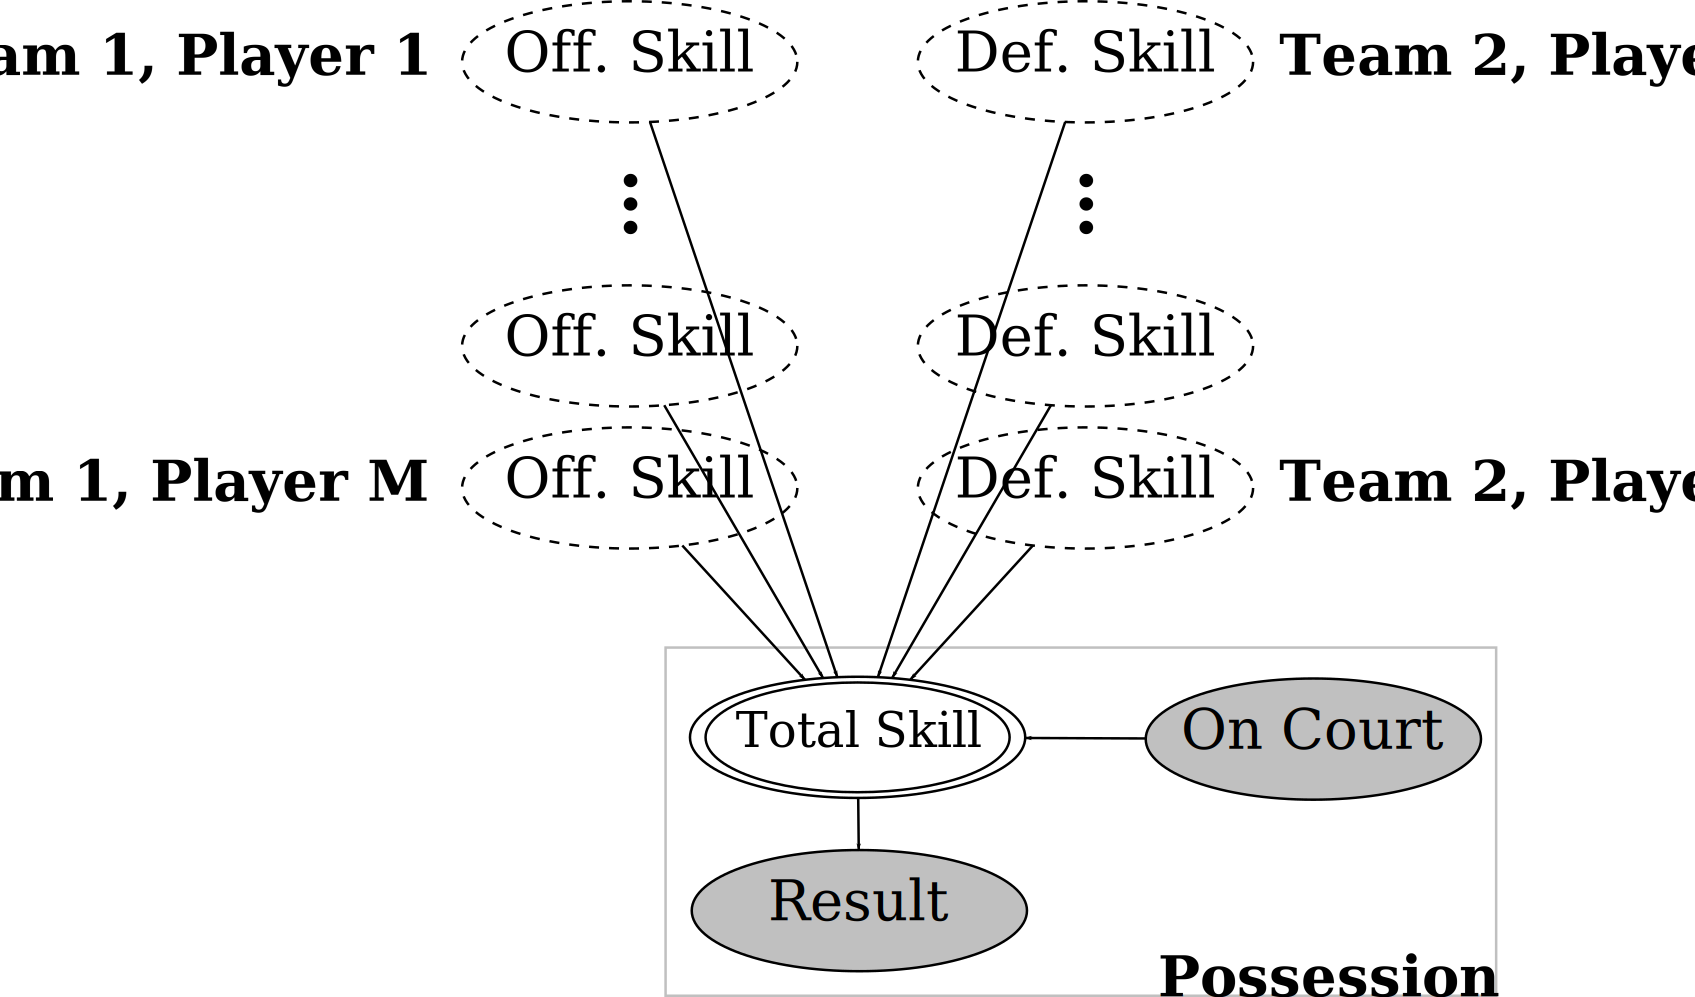
\includegraphics[width=0.90\linewidth]{figures/network}
\end{center}
These skills would contribute deterministically in some way to an ``effective'' total skill differential between the two teams, and then the \emph{Result} variable would be one of four outcomes:
\begin{itemize}
\item $R=0$ Offensive Team Scores nothing, change of possession (e.g. turnover, defensive rebound, etc.)
\item $R=1$ Offensive Team Scores 1 point
\item $R=2$ Offensive Team Scores 2 points
\item $R=3$ Offensive Team Scores 3 points
\end{itemize}

The \emph{On Court} random variable ``multiplexes'' between those players that are on the court and those that are not.

\subsection{Issues}
\label{sec:badnetwork}
These traditional models~\cite{herbrich2007trueskilltm} have difficulty capturing the proper causalities when Results can have multinomial-valued outcomes.
For example, regardless of the parameterization of the \emph{Results} CPD, both $\prb{ R = 2}$ and $\prb{R= 3}$ would depend on the same skills of the same players.
The relative distribution of outcomes $\prb{R = 2}$ vs. $\prb{R = 3}$ would be shared across all ``units'' (i.e. all combinations of \emph{On Court} assignments).

In reality, a team that scores $R=3$ half the time and $R=1$ half the time is just as good as a team that scores $R=2$ all the time.
However, any traditional Win/Lose model will unfairly penalize the likelihood of one of these teams over the other and leads to under-fitting.
This might suggest that we have a random variable that represents $\Elin{\mathrm points scored}$, but this doesn't pass the clarity test.


Secondly, there is a lot of value in being able to compare with the state-of-the-art in the Win/Lose based Bayesian Skill Ranking literature.
Specifically, there is common debate over logistic vs. Gaussian skill/performance distributions and we wish to be sensitive to that conversation in this project.
Having a multinomial outcome makes it difficult to directly compare logistic vs. Gaussian in the standard skill/performance framework because there is no consensus in the literature about how to extend these models just to support ties~\cite{hunter2004mm}, let alone general multinomial outcomes.

\subsection{Proposed Network}

To address some of the shortcomings discussed in {\bf Section~\ref{sec:badnetwork}}, we propose the following:
\begin{center}
	
\includegraphics[width=1.05\linewidth]{figures/newnetwork}
\end{center}

In this network, each player is represented by three skill parameters:
\begin{enumerate}
\item Skill 1: Ability to score (or defend against) one-point opportunities
\item Skill 2: Ability to score (or defend against) two-point opportunities
\item Skill 3: Ability to score (or defend against) three-point opportunities
\end{enumerate}

On each possession, there are three binary hidden random variables:
\begin{enumerate}
\item \emph{Win 1}: True if there was an opportunity to score one point during the possession.
\item \emph{Win 2}: True if there was an opportunity to score two points during the possession.
\item \emph{Win 3}: True if there was an opportunity to score three points during the possession.
\end{enumerate}

Now, \emph{Result} simply selects the highest-valued scoring opportunity available during the possession.
If \emph{Win 3} is true, \emph{Result} is 3; If \emph{Win 3} is false but \emph{Win 2} is true, \emph{Result} is 2; etc.

\emph{Result} can be specified with either a tree-CPD or table-CPD, but it has the following probabilities.

\begin{tabular}{ l|r r r r}
 & $R=0$ & $R=1$ & $R=2$ & $R=3$ \\  \hline
$w^1_3 w^1_2 w^1_1$ & $\varepsilon$ &  $\varepsilon$ &  $\varepsilon$ & $(1 - 3 \varepsilon)$ \\ \hline
\end{tabular}

The single parameter $\varepsilon$ is inspired by the noisy-max and essentially indicates unmodelled errors (e.g. offensive or defensive mistakes).
The better our model fits the actual flow of the game, the smaller $\varepsilon$ should be.

\section{Implemention}

Summary

\section{Results}

Data

\section{Analysis}

Details

\section{Conclusions}

Done


\section{References}
%\small{
\bibliographystyle{ieeetran}
\bibliography{ieeeabrv,references/references}
%\bibliography{references/references}
%}

\end{document}